\chapter{Performance comparison}

This report will use the MATLAB profiler to discuss the runtime performance of MATLAB code implementations of the Block MLDU algorithm. The runtime of a piece of code is dependent on both the efficiency of the code and the hardware on which it is executed. This means that the runtime performance results will most likely vary from computer to computer. In order to verify if the achieved results on any given computer are in line with expectations, one must also be able to compare the general MATLAB related performance of the computer.\\

\noindent MATLAB provides a means to achieve this comparison by way of the \texttt{bench()} function. It runs a micro-benchmark with a variety of "typical" MATLAB workloads, namely:

\begin{itemize}
    \item LU decomposition
    \item FFT
    \item ODE with \texttt{ode45}
    \item Sparse
    \item 2D
    \item 3D
\end{itemize}

\noindent The most important benchmarks for this algorithm are LU decomposition, FFT and Sparse, because they touch on hardware performance elements that are similar to the the Block MLDU algorithm. More information can be found by running: \texttt{doc bench}\\

\noindent It should be noted that these benchmarks are far from an ideal way to compare different computers, but it can give a rough indication. It is recommended to run the benchmarks at least $10$ times, as there can be some significant performance variance.

\section{Test machine hardware specifications}

A more detailed performance comparison between computers requires the hardware specifications. The test machine specifications are provided below:

\begin{itemize}
    \item CPU: Intel Xeon E5-1650 v3 6 core 12 thread overclocked to 3.8 GHz
    \item Memory: 32 GB 4 channel DDR4 registered ECC running at 2133 MHz.
    \item Graphics: Two NVIDIA GTX Titan (Kepler) running in SLI
\end{itemize}

\newpage

\section{Test machine benchmark results}

\begin{figure}[h!]
    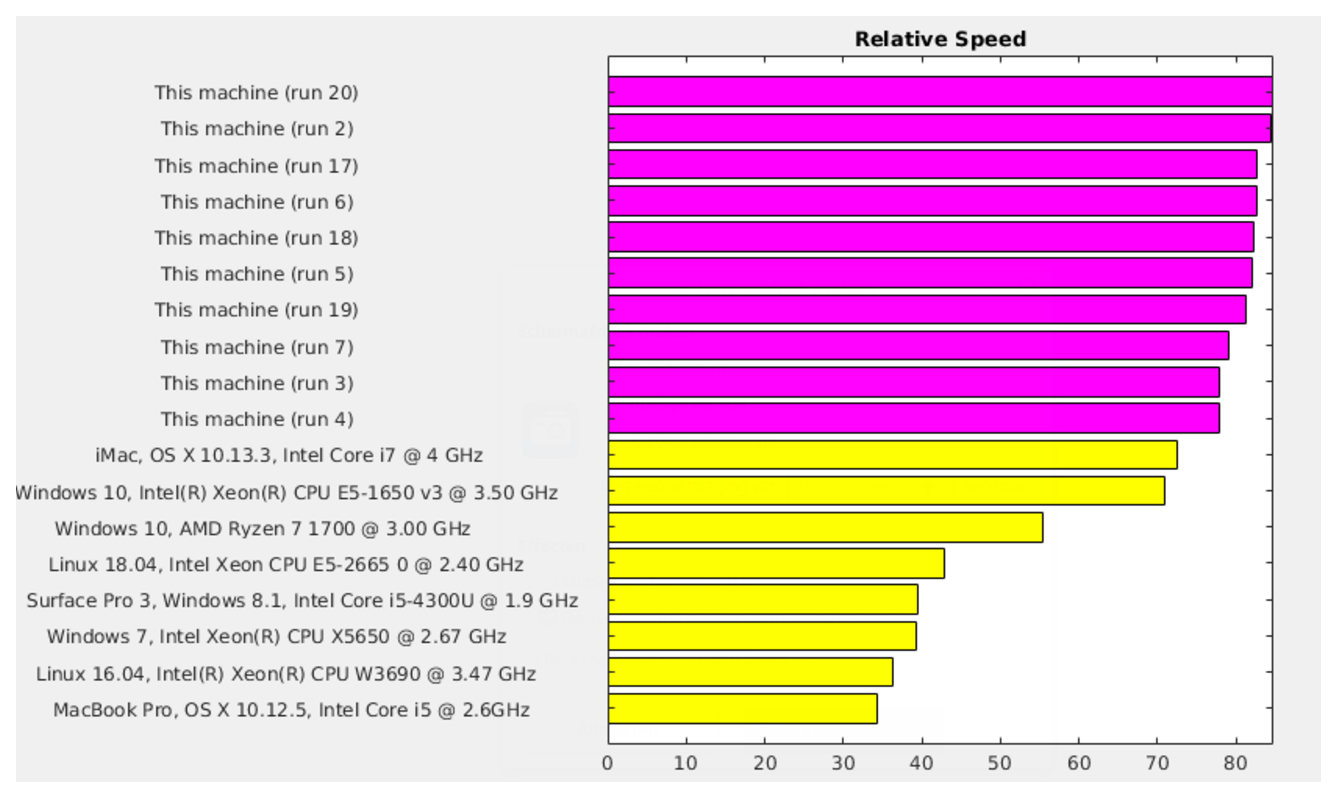
\includegraphics[width=\linewidth]{figures/Performance_1.eps}
    \centering
\end{figure}

\begin{figure}[h!]
    \includegraphics[width=\linewidth]{figures/Performance_2.eps}
    \centering
\end{figure}

\noindent As can bee seen, the performance of the test machine is generally very high. The second thing to note is that the performance varies quite significantly, sometimes as much as about $33 \%$. That is why this benchmark was run $20$ times, even though it only shows the results from the $10$ best runs.